\documentclass[12pt,fleqn]{article}\usepackage{../common}
\begin{document}
Dinamik Programlama

Dinamik programlamanin (DP) temelinde ardi ardina verilmesi gereken
kararlarin bulunmasi fikri yatar; her anda, her verilen karar baska bir
karar secenekleri ortaya cikarabilir, ve bunlarin arasinda da secim
yapilmalidir. Hedefimiz en iyi karar zincirini bulmaktir. Bu kismen
``acgozlu algoritmalar (greedy algorithms)'' olarak bilinen algoritmalarin
yaptigina benzer, fakat acgozlu algoritmalar, mesela en kisa yolu bulmaya
ugrasirken gezilen dugumlerde sadece ``o an icin' en iyisini yapar; Bu
yaklasimin problemi o an icin iyi olan toplam goze alindigi zaman en iyi
sonucu olmayabilecegidir; Mesela alttaki grafige bir bakalim,

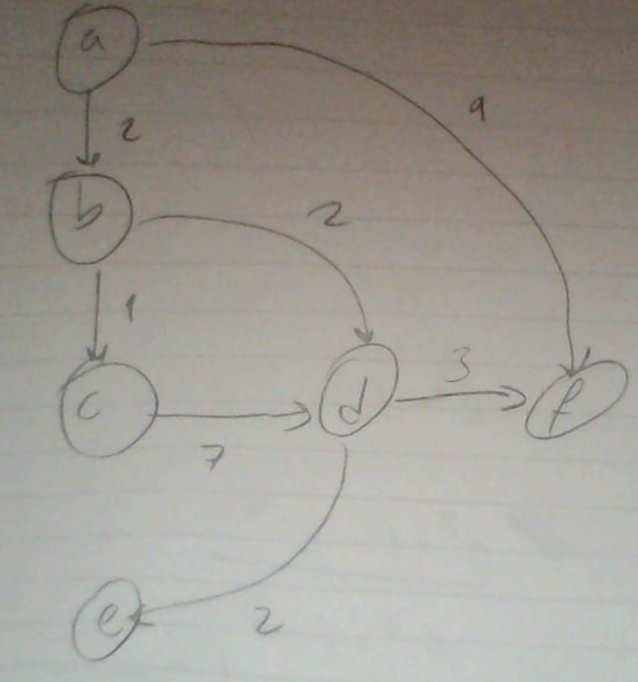
\includegraphics[height=6cm]{dp1.jpg}

Diyelim ki \verb!a! noktasindan \verb!f! noktasina en kisa yoldan ulasmaya
calisiyoruz. Acgozlu algoritma \verb!a,b,c,d! uzerinden gidis yapardi cunku
her an, sadece ``o an icin'' en iyi olani secerdi. Fakat toplama bakarsak,
bu yolun en kisa yol olmadigini goruruz. En iyi yol \verb!a,b,d! uzerinden
giden yoldur.

Ustteki cizit, ag yapisi (graph) yonlu, �evrimsiz (directed, acyclic graph
-DAG-) diye bilinen bir yapidir. Tipik kisa yol problemleri bu yapilar
uzerinde calisirlar. 

DP problemleri bir problemi alt problemlere bolebildigimiz zaman
faydalidirlar ve ozellikle o alt problemler cogunlukla tekrar tekrar
hesaplaniyorlarsa iyidir, cunku DP o alt problemleri onbellekleyerek tekrar
hesaplanmadan gecilmelerini saglayabilir. 

Ornek olarak en kisa yol problemini DP ile cozelim. 

Problemin tamami, teorik ve tumevarimsal olarak biraz dusunelim. Diyelim ki
ustteki DAG'de $a,f$ arasindaki en kisa yolu kesin biliyoruz. Ve yine
diyelim ki bu yol uzerinde / bir ara nokta $x$ noktasi var. O zaman, $a,x$,
ve $x,f$ arasindaki yollar da tanim itibariyle en kisadir. Ispat: eger
mesela $x,f$ arasindaki en kisa yol bildigimizden baska olsaydi, o zaman
eldekini atip o yolu kullaniyor olurduk, ve bu sefer bu alternatif en kisa
olurdu. Fakat ilk basta en kisa yolu bildigimiz faraziyesi ile
basladik. Bir celiski elde ettik, demek ki ara noktanin kisaligi dogrudur
$\square$

Bu ispattan / bilgiden hareketle, kisa yolu tek numerik bir deger olarak
hesaplamaya ugrasalim. 

Oyle bir fonksiyon $d(v)$ olsun ki herhangi bir $v$ nodu icin o nod'dan
bitis noktasina olan en kisa uzakligi hesaplayabiliyor olsun, $u,v$
arasindaki parca mesafeler ise $w(u,v)$ ile verilecek. 

Veri yapisi olarak DAG'i alttaki gibi gosterelim,

\begin{minted}{python}
DAG = {
    'a': {'b':2, 'f': 9},
    'b': {'d':2, 'c':1, 'f': 6},
    'c': {'d':7},
    'd': {'e':2, 'f': 3},
    'e': {'f':4},
    'f': {}
}
\end{minted}

Boylece $w(u,v)$ basit bir Python sozluk (dictionary) erisimi haline
geliyor, mesela \verb!a,b! arasi parca mesafe icin 

\begin{minted}{python}
print DAG['a']['b']
\end{minted}

\begin{verbatim}
2
\end{verbatim}

En kisa yolu bulacak program

\begin{minted}{python}
from functools import wraps

def memo(func):
    cache = {}                                  
    @wraps(func)                                
    def wrap(*args):                            
        if args not in cache:
            print 'miss', args[0]
            cache[args] = func(*args)
        else: print 'hit for', args[0]
        return cache[args]                      
    return wrap 

def rec_dag_sp(W, s, t): 
    @memo                                    
    def d(u):
        print ('At ' + u[0])
        if u == t: return 0                     
        dist = min(W[u][v]+d(v) for v in W[u])  
        print 'returning from',u,', dist=',dist
        return dist
    return d(s)                                 

dist = rec_dag_sp(DAG, 'a', 'f')
print 'final distance=', dist
\end{minted}

\begin{verbatim}
miss a
At a
miss b
At b
miss c
At c
miss d
At d
miss e
At e
miss f
At f
returning from e , dist= 4
hit for f
returning from d , dist= 3
returning from c , dist= 10
hit for d
hit for f
returning from b , dist= 5
hit for f
returning from a , dist= 7
final distance= 7
\end{verbatim}

\end{document}
